\documentclass[10pt,paper=a5,pagesize]{scrbook}
\usepackage{geometry}
\usepackage{fontspec}                           
\usepackage{graphicx}
\usepackage{tcolorbox}
\usepackage[french]{babel}
\usepackage{tikz}
\usepackage{rubikcube,rubikrotation}
\usepackage{parskip}
\usepackage{enumitem}
\usepackage{pdfpages}
\usepackage{url}
\usepackage[nochapter]{vhistory}


\usetikzlibrary{arrows}
\setlist[itemize,1]{label={\fontfamily{cmr}\fontencoding{T1}\selectfont\textbullet}}

\setmainfont{Alegreya Sans}

\newfontfamily\barlow{Barlow Semi Condensed}
\setkomafont{disposition}{\barlow}

\begin{document}
\frontmatter
\thispagestyle{empty}

\begin{titlepage}
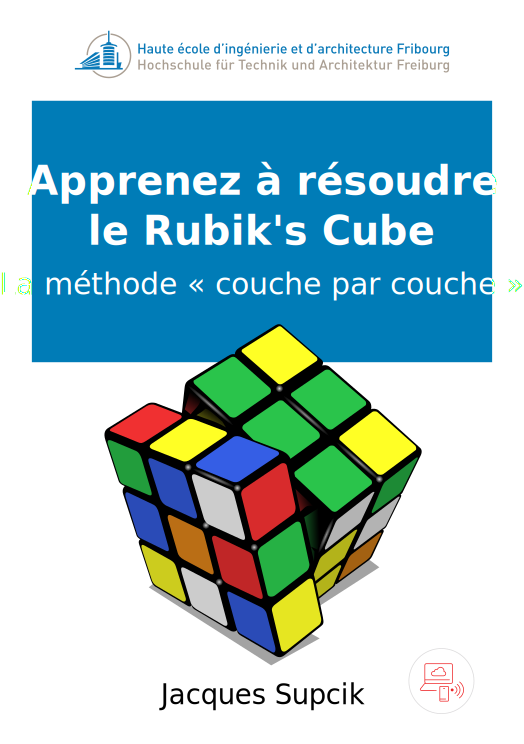
\includepdf{title}
\end{titlepage}

\thispagestyle{empty}
\null
\vfill

Le code source de ce document est disponible sur github à l'adresse\\
\url{https://github.com/supcik/manuel-rubik-cube-fr}.
\par\vspace*{8mm}

\begin{minipage}[c]{\textwidth}
\begin{versionhistory}
	\vhEntry{1.0.3}{5.06.2022}{JS}{Corrections mineures}
	\vhEntry{1.0.2}{20.06.2019}{JS}{Nouvelle page de titre}
	\vhEntry{1.0.1}{17.06.2019}{JS}{Corrections}
	\vhEntry{0.0.0}{20.02.2016}{JS}{Première ébauche}
\end{versionhistory}
\end{minipage}
\par\vspace*{10mm}



\includegraphics[width=30mm]{by.pdf}

Copyright \textcopyright{} 2022 Jacques Supcik

Cette œuvre est mise à disposition selon les termes de la Licence Creative Commons Attribution 4.0 International.
\medskip\\
Pour obtenir une copie de la licence, visitez:\\
\url{http://creativecommons.org/licenses/by/4.0/deed.fr}.
\newpage

\tableofcontents
\chapter*{Remerciements}

Merci à tous ceux qui ont contribué à la réalisation de ce livre. Merci à Pascal Supcik pour la relecture du manuscrit et la correction de nombreuses erreurs. Merci à Milena Supcik, Damien Goetschi et Baptiste Wicht pour avoir testé les méthodes lors des ateliers avec les enfants. Merci enfin à tous les enfants qui ont utilisé une première version de ce livre et qui m'ont permis d'améliorer certains passages.
\mainmatter
\chapter{Introduction}

Le Rubik's cube a été inventé en 1974 par le sculpteur et professeur d'architecture hongrois \emph{Ernő Rubik}. Pour la petite histoire, il a fallu plus d'un mois à Ernő Rubik pour résoudre sa propre invention! Ce cube était très populaire
dans les années~80, et aujourd'hui encore, il reste un objet très apprécié
par tous ceux qui s'intéressent aux sciences, aux mathématiques, ou à la technologie.

Les règles du jeu sont extrêmement simples: il suffit de faire pivoter les parties du cube de manière à rassembler toutes les pastilles de la même couleur sur la même face:

\begin{center}
	\RubikCubeSolved
	\ShowCube{2cm}{0.5}{%
		\DrawRubikCubeRU
	}
\end{center}


Mais la simplicité s'arrête là. En effet, il y a plus de 43~trillions\footnote{Pour être précis, il y a 43\,252\,003\,274\,489\,856\,000 configurations possibles.} configurations possibles du cube et il est très difficile de prévoir quels mouvements seront nécessaires pour résoudre un cube bien «mélangé».

Des chercheurs ont démontré\cite{god20} qu'on pouvait résoudre n'importe quel cube avec un maximum de 20~mouvements. La méthode \emph{couche par couche} présentée dans ce livre nécessite beaucoup plus que 20~mouvements, mais elle a l'avantage d'être bien adaptée aux débutants. Si, plus
tard, vous souhaitez battre des records de vitesse, vous devrez apprendre
d'autres méthodes; plus rapides, mais aussi plus difficiles à mémoriser.
 
Nous commencerons par positionner toutes les pièces de la couche du haut, ensuite nous positionnerons les pièces de la couche du milieu et nous terminerons par les pièces de la dernière
couche. Prenez le temps de bien exercer chaque couche avant de passer
à la suivante. Vous n'apprendrez pas plus vite en brûlant les étapes. Si vous utilisez ce livre dans le cadre d'une série d'ateliers, vous pouvez très bien faire trois
séances de une heure chacune. Vous étudierez alors une couche par séance et vous aurez du temps pour vous exercer entre les séances. 


\chapter{Les différentes parties du cube}

Commençons par étudier les différentes parties du Rubik's cube.

\section{Les centres}

Le cube se compose de 6~\textbf{centres} qui sont toujours placés de la même manière:

\begin{center}
	\RubikFaceUp%
	{X}{X}{X}%
	{X}{W}{X}%
	{X}{X}{X}
	\RubikFaceRight%
	{X}{X}{X}%
	{X}{G}{X}%
	{X}{X}{X}
	\RubikFaceFront%
	{X}{X}{X}%
	{X}{O}{X}%
	{X}{X}{X}
	\ShowCube{2cm}{0.5}{%
		\DrawRubikCubeRU
	}
\end{center}

Les centres sont identifiés par une \textbf{pastille}\footnote{La plupart des cubes du commerce ont des auto-collants pour identifier les couleurs}. Les
couleurs du cube original sont blanc, rouge, bleu, orange, vert et
jaune. Si votre cube a d'autres couleurs, ce n'est pas grave, la méthode
reste la même.

Les centres restent toujours à la même place; vous pouvez faire tous les
mouvements que vous voulez, vous ne changerez jamais la position des
centres.

\section{Les arêtes}
\begin{samepage}
Le cube se compose également de 12~\textbf{arêtes}:

\begin{center}
	\RubikFaceUp%
	{X}{W}{X}%
	{W}{X}{W}%
	{X}{W}{X}
	\RubikFaceRight%
	{X}{G}{X}%
	{G}{X}{G}%
	{X}{G}{X}
	\RubikFaceFront%
	{X}{O}{X}%
	{O}{X}{O}%
	{X}{O}{X}
	\ShowCube{2cm}{0.5}{%
		\DrawRubikCubeRU
	}
\end{center}
\end{samepage}

Les arêtes sont les pièces placées entre les centres et elles ont toutes
2~pastilles de couleurs différentes.

\section{Les sommets}

Pour terminer, le cube a 8~\textbf{sommets}:

\begin{center}
	\RubikFaceUp%
	{W}{X}{W}%
	{X}{X}{X}%
	{W}{X}{W}
	\RubikFaceRight%
	{G}{X}{G}%
	{X}{X}{X}%
	{G}{X}{G}
	\RubikFaceFront%
	{O}{X}{O}%
	{X}{X}{X}%
	{O}{X}{O}
	\ShowCube{2cm}{0.5}{%
		\DrawRubikCubeRU
	}
\end{center}

Chaque sommet a 3~pastilles de couleurs différentes.

Il reste encore une pièce que nous ne voyons pas et qui est au milieu du
cube. Si on additionne tous les types de pièces, on a $6 + 12 + 8 + 1 =
27$, ce qui correspond bien à ce que nous attendions avec un cube de $3
\times 3 \times 3$.

\section{Les couches}
\begin{samepage}
Une \textbf{couche} peut être comparée à un «étage» du cube. Le Rubik's cube est composé de trois couches:

\begin{center}
	\RubikFaceUp%
	{W}{W}{W}%
	{W}{W}{W}%
	{W}{W}{W}
	\RubikFaceRight%
	{G}{G}{G}%
	{X}{X}{X}%
	{X}{X}{X}
	\RubikFaceFront%
	{O}{O}{O}%
	{X}{X}{X}%
	{X}{X}{X}
	\ShowCube{2cm}{0.5}{%
		\DrawRubikCubeRU
		\node[anchor=center] at(1.5,2.5) {1};
	}
	\hspace*{5mm}
	\RubikFaceUp%
	{X}{X}{X}%
	{X}{X}{X}%
	{X}{X}{X}
	\RubikFaceRight%
	{X}{X}{X}%
	{G}{G}{G}%
	{X}{X}{X}
	\RubikFaceFront%
	{X}{X}{X}%
	{O}{O}{O}%
	{X}{X}{X}
	\ShowCube{2cm}{0.5}{%
		\DrawRubikCubeRU
		\node[anchor=center] at(1.5,1.5) {2};
	}
	\hspace*{5mm}
	\RubikFaceUp%
	{X}{X}{X}%
	{X}{X}{X}%
	{X}{X}{X}
	\RubikFaceRight%
	{X}{X}{X}%
	{X}{X}{X}%
	{G}{G}{G}
	\RubikFaceFront%
	{X}{X}{X}%
	{X}{X}{X}%
	{O}{O}{O}
	\ShowCube{2cm}{0.5}{%
		\DrawRubikCubeRU
		\node[anchor=center] at(1.5,0.5) {3};
	}
\end{center}
\end{samepage}
	
Avec la méthode proposée dans ce livre, vous commencerez par faire la
première couche (parfois aussi appelée couche du haut), puis vous
passerez à la deuxième couche (ou couche du milieu) et vous terminerez
avec la troisième couche (ou couche du bas).

\section{Les faces}

\begin{center}
	\RubikFaceUp%
	{W}{W}{W}%
	{W}{W}{W}%
	{W}{W}{W}
	\RubikFaceRight%
	{X}{X}{X}%
	{X}{X}{X}%
	{X}{X}{X}
	\RubikFaceFront%
	{X}{X}{X}%
	{X}{X}{X}%
	{X}{X}{X}
	\ShowCube{2cm}{0.5}{%
		\DrawRubikCubeRU
	}
	\hspace*{5mm}
	\RubikFaceUp%
	{X}{X}{X}%
	{X}{X}{X}%
	{X}{X}{X}
	\RubikFaceRight%
	{G}{G}{G}%
	{G}{G}{G}%
	{G}{G}{G}
	\RubikFaceFront%
	{X}{X}{X}%
	{X}{X}{X}%
	{X}{X}{X}
	\ShowCube{2cm}{0.5}{%
		\DrawRubikCubeRU
	}
	\hspace*{5mm}
	\RubikFaceUp%
	{X}{X}{X}%
	{X}{X}{X}%
	{X}{X}{X}
	\RubikFaceRight%
	{X}{X}{X}%
	{X}{X}{X}%
	{X}{X}{X}
	\RubikFaceFront%
	{O}{O}{O}%
	{O}{O}{O}%
	{O}{O}{O}
	\ShowCube{2cm}{0.5}{%
		\DrawRubikCubeRU
	}
\end{center}


\chapter{La première couche}

{
\centering
\RubikFaceUpAll{W}
\RubikFaceRight%
{G}{G}{G}%
{X}{G}{X}%
{X}{X}{X}
\RubikFaceFront%
{O}{O}{O}%
{X}{O}{X}%
{X}{X}{X}
\ShowCube{4cm}{1}{%
	\DrawRubikCubeRU
}
\par
}
\medskip

Pour commencer, nous allons résoudre la couche du haut du cube. Nous choisissons de positionner
le cube avec le centre blanc vers le haut, mais vous pouvez choisir une autre couleur si vous préférez.


\section{La croix}

Pour résoudre la première couche du cube, nous commençons
par faire une «croix» sur la face du haut.

\begin{center}
\RubikFaceUp%
{X}{W}{X}%
{W}{W}{W}%
{X}{W}{X}
\RubikFaceRight%
{X}{G}{X}%
{X}{G}{X}%
{X}{X}{X}
\RubikFaceFront%
{X}{O}{X}%
{X}{O}{X}%
{X}{X}{X}
\ShowCube{2cm}{0.5}{%
	\DrawRubikCubeRU
}
\end{center}

Notez qu'il ne suffit pas de mettre les 4 arrêtes blanches sur la face du haut, il faut aussi
que l'autre côté des arrêtes corresponde avec la couleur des autres centres (orange et vert dans l'exemple ci-dessus).

Cette première couche peut se résoudre de manière assez intuitive et certains n'auront pas besoin
d'aide. Voici cependant des indications pour ceux qui auraient plus de peine.

Notez que vous pouvez faire pivoter la couche du bas de votre cube tant que vous voulez sans «casser» ce que vous avez déjà fait sur les couches du haut. \rrh{D} ou \rrh{Dp}. Ca nous sera bien utile pour la suite.

\subsection{L'arrête à déplacer se trouve sur la dernière couche}
\label{subsec:c1d}

Si l'arrête que vous souhaitez déplacer pour faire la croix se trouve sur la couche du bas, vous pouvez tourner cette couche du bas pour l'amener sur la bonne face. Nous aurons alors deux cas possible:

Soit l'arrête a la face blanche vers le bas:

\begin{center}
	\RubikFaceDown%
	{X}{W}{X}%
	{X}{Y}{X}%
	{X}{X}{X}
	\RubikFaceRight%
	{X}{X}{X}%
	{X}{G}{X}%
	{X}{X}{X}
	\RubikFaceFront%
	{X}{X}{X}%
	{X}{O}{X}%
	{X}{O}{X}
	\ShowCube{2cm}{0.5}{%
		\DrawRubikCubeRD
	}
\end{center}

et dans ce cas il suffit de faire tourner la face avant deux fois: \rrh{F}\rrh{F} (ou \rrh{Fp}\rrh{Fp}).

Ou alors l'arrête blanche est sur la face avant:

\begin{center}
	\RubikFaceDown%
	{X}{O}{X}%
	{X}{Y}{X}%
	{X}{X}{X}
	\RubikFaceRight%
	{X}{X}{X}%
	{X}{G}{X}%
	{X}{X}{X}
	\RubikFaceFront%
	{X}{X}{X}%
	{X}{O}{X}%
	{X}{W}{X}
	\ShowCube{2cm}{0.5}{%
		\DrawRubikCubeRD
	}
\end{center}

Dans ce cas, nous faisons remonter l'arrête avec les mouvements suivants: \rrh{D}\rrh{Sl}\rrh{Dp}\rrh{Slp}


\subsection{L'arrête se trouve sur la couche du milieu}

Si l'arrête se trouve sur la couche du milieu, comme ceci:

\begin{center}
	\RubikFaceUp%
	{X}{X}{X}%
	{X}{W}{X}%
	{X}{X}{X}
	\RubikFaceRight%
	{X}{X}{X}%
	{W}{G}{X}%
	{X}{X}{X}
	\RubikFaceFront%
	{X}{X}{X}%
	{X}{O}{O}%
	{X}{X}{X}
	\ShowCube{2cm}{0.5}{%
		\DrawRubikCubeRU
	}
\end{center}

On peut amener cette arrête en place tout simplement en tournant la face avant dans le sens anti-horaire\footnote{Dans le sens contraire des aiguilles d'une montre}: \rrh{Fp}.

Si l'arrête se trouve sur la face du milieu, mais qu'elle est mal positionnée

\begin{center}
	\RubikFaceUp%
	{X}{X}{X}%
	{X}{W}{X}%
	{X}{X}{X}
	\RubikFaceRight%
	{X}{X}{X}%
	{O}{G}{X}%
	{X}{X}{X}
	\RubikFaceFront%
	{X}{X}{X}%
	{X}{O}{W}%
	{X}{X}{X}
	\ShowCube{2cm}{0.5}{%
		\DrawRubikCubeRU
	}
\end{center}

alors on peut déplace cette arrête sur la couche du bas: \rrh{Rp}\rrh{Dp}\rrh{R} et on ramène l'arrête correctement positionnée sur la couche du haut: \rrh{F}\rrh{F}


Si l'arrête se trouve sur la couche du milieu, mais nêst pas sur la bonne face:

\begin{center}
	\RubikFaceUp%
	{X}{X}{X}%
	{X}{W}{X}%
	{X}{X}{X}
	\RubikFaceRight%
	{X}{X}{X}%
	{W}{R}{X}%
	{X}{X}{X}
	\RubikFaceFront%
	{X}{X}{X}%
	{X}{G}{O}%
	{X}{X}{X}
	\ShowCube{2cm}{0.5}{%
		\DrawRubikCubeRU
	}
\end{center}

alors on déplace cette arrête sur la couche du bas: \rrh{F}\rrh{Dp}\rrh{Fp} et on applique la règle pour la couche du bas comme expliqué en \ref{subsec:c1d}.


Pour gagner du temps, lorsqu'on déplace une arrête sur la couche du bas, on va positioner l'arrête de manière à ce que sa face blanche soit vers le bas. C'est le cas pour l'exemple ci-dessus.

Si l'arrête de positionnée comme dans le cube ci-dessous:

\begin{center}
	\RubikFaceUp%
	{X}{X}{X}%
	{X}{W}{X}%
	{X}{X}{X}
	\RubikFaceRight%
	{X}{X}{X}%
	{O}{R}{X}%
	{X}{X}{X}
	\RubikFaceFront%
	{X}{X}{X}%
	{X}{G}{W}%
	{X}{X}{X}
	\ShowCube{2cm}{0.5}{%
		\DrawRubikCubeRU
	}
\end{center}

Alors on fait: \rrh{Rp}\rrh{Dp}\rrh{R}

\subsection{L'arrête se trouve sur la couche du haut}

Si l'arrête se trouve sur la couche du haut mais que ses couleurs sont inversés, comme dans l'exemple ci-dessous:

\begin{center}
	\RubikFaceUp%
	{X}{X}{X}%
	{X}{W}{X}%
	{X}{O}{X}
	\RubikFaceRight%
	{X}{X}{X}%
	{X}{G}{X}%
	{X}{X}{X}
	\RubikFaceFront%
	{X}{W}{X}%
	{X}{O}{X}%
	{X}{X}{X}
	\ShowCube{2cm}{0.5}{%
		\DrawRubikCubeRU
	}
\end{center}

On peut faire pivoter l'arrête avec la séquence suivante: \rrh{F}\rrh{F}\rrh{D}\rrh{Sl}\rrh{Dp}\rrh{Slp}.

Les deux premiers mouvements mettent l'arrête sur la dernière couche et la suite est la même séquence que dans la section \ref{subsec:c1d}.

\begin{samepage}
Si l'arrête est déjà bien orientée, mais qu'elle n'est pas au bon endroit, comme dans l'exemple ci-dessous:

\begin{center}
	\RubikFaceUp%
	{X}{X}{X}%
	{X}{W}{W}%
	{X}{X}{X}
	\RubikFaceRight%
	{X}{O}{X}%
	{X}{G}{X}%
	{X}{X}{X}
	\RubikFaceFront%
	{X}{X}{X}%
	{X}{O}{X}%
	{X}{X}{X}
	\ShowCube{2cm}{0.5}{%
		\DrawRubikCubeRU
	}
\end{center}
\end{samepage}


Si c'est la première arrête que vous mettez en place, vous pouvez simplement tourner la face du haut: \rrh{U}, mais si les autres arrêtes sont déjà en place, vous pouvez alors amener l'arrête sur la dernière couche: \rrh{Rp}\rrh{Rp}. L'arrête se trouve alors sur la dernière couche et on applique la méthode expliqué en \ref{subsec:c1d}.

Si l'arrête se trouve sur la dernière couche et qu'elle n'est ni bien orientée, ni bien positionnée:

\begin{center}
	\RubikFaceUp%
	{X}{X}{X}%
	{X}{W}{O}%
	{X}{X}{X}
	\RubikFaceRight%
	{X}{W}{X}%
	{X}{G}{X}%
	{X}{X}{X}
	\RubikFaceFront%
	{X}{X}{X}%
	{X}{O}{X}%
	{X}{X}{X}
	\ShowCube{2cm}{0.5}{%
		\DrawRubikCubeRU
	}
\end{center}

Vous pouvez l'ammener sur la couche du bas: \rrh{Rp}\rrh{Rp}\rrh{Dp}\rrh{R}\rrh{R} et ensuite appliquer la méthode expliqué en \ref{subsec:c1d}.

Notez que dans l'exemple ci dessus, vous pouvez mettre l'arrête en place en continuant avec la simple séquence suivante: \rrh{Rp}\rrh{Fp}

\section{Les coins de la première couche}

Pour terminer la première couche, il ne nous reste plus qu'à mettre les coins en place.

\subsection{Le coin à déplacer se trouve sur la couche du bas}
\label{subsec:c1cd}

Si le coin se trouve sur la dernière couche, il y a trois cas possibles.
Le premier cas est celui où le coin est placé avec la côté blanc vers
la face et il doit monter en diagonale: 

\begin{center}  	
	\RubikFaceRight%
	{X}{G}{X}%
	{X}{G}{X}%
	{X}{X}{X}
	\RubikFaceFront%
	{X}{O}{X}%
	{X}{O}{X}%
	{W}{X}{X}
	\RubikFaceDown%
	{G}{X}{X}%
	{X}{Y}{X}%
	{X}{X}{X}
	
	\ShowCube{2cm}{0.5}{%
		\DrawRubikCubeRD
		\tikzset{>=latex}
		\draw[thick,->] (0.5,0.5) -- (2.5,2.5);
	}
\end{center} 

On résout ce cas avec la séquence suivante:
\rrh{D}\rrh{D}\rrh{F}\rrh{Dp}\rrh{Fp}

Le deuxième cas est celui où le coin est placé avec la côté blanc vers
la face et il doit monter en verticale: 

\begin{center}
	\RubikFaceRight%
	{X}{G}{X}%
	{X}{G}{X}%
	{G}{X}{X}
	\RubikFaceFront%
	{X}{O}{X}%
	{X}{O}{X}%
	{X}{X}{W}
	\RubikFaceDown%
	{X}{X}{O}%
	{X}{Y}{X}%
	{X}{X}{X}
	
	\ShowCube{2cm}{0.5}{%
		\DrawRubikCubeRD
		\tikzset{>=latex}
		\draw[thick,->] (2.5,0.5) -- (2.5,2.5);
	}
\end{center} 

On résout ce cas avec la séquence suivante:
\rrh{Dp}\rrh{Rp}\rrh{D}\rrh{R}


Le troisième cas est celui où le coin est placé avec la côté blanc vers
le bas. On commence par placer le coin à la verticale de la position
vers laquelle on souhaite l'amener:

\begin{center}
	\RubikFaceRight%
	{X}{G}{X}%
	{X}{G}{X}%
	{O}{X}{X}
	\RubikFaceFront%
	{X}{O}{X}%
	{X}{O}{X}%
	{X}{X}{G}
	\RubikFaceDown%
	{X}{X}{W}%
	{X}{Y}{X}%
	{X}{X}{X}
	
	\ShowCube{2cm}{0.5}{%
		\DrawRubikCubeRD
		\tikzset{>=latex}
		\draw[thick,<->] (2.5,0.5) -- (2.5,2.5);
	}
\end{center} 

La séquence suivante permet de faire pivoter le coin et le mettre en bas à gauche: \rrh{Rp}\rrh{D}\rrh{D}\rrh{R}

\begin{samepage}
Le résultat sera:

\begin{center}
	\RubikFaceRight%
	{X}{G}{X}%
	{X}{G}{X}%
	{X}{X}{X}
	\RubikFaceFront%
	{X}{O}{X}%
	{X}{O}{X}%
	{W}{X}{X}
	\RubikFaceDown%
	{G}{X}{X}%
	{X}{Y}{X}%
	{X}{X}{X}
	
	\ShowCube{2cm}{0.5}{%
		\DrawRubikCubeRD
	}
\end{center} 
\end{samepage}
	
Ce qui correspond à un cas connu et nous savons alors comment le faire
venir à sa position finale.

\subsection{Le coin à déplacer se trouve sur la face du haut}

Les coins peuvent déjà se trouver soit sur la couche du haut, mais leur
position n'est peut-être pas la bonne.

Pour déplacer un coin, nous devons commencer par l'amener sur la couche du bas. Prenons l'exemple du cube ci-dessous:

\begin{center}
	\RubikFaceUp%
	{X}{W}{X}%
	{W}{W}{W}%
	{X}{W}{G}
	\RubikFaceRight%
	{O}{R}{X}%
	{X}{R}{X}%
	{X}{X}{X}
	\RubikFaceFront%
	{X}{G}{W}%
	{X}{G}{X}%
	{X}{X}{X}
	\ShowCube{2cm}{0.5}{%
		\DrawRubikCubeRU
	}
\end{center}

Nous avons 4 possibilités pour faire descendre ce coin sur la dernière couche:

\begin{itemize}
	\item \rrh{F}\rrh{D}\rrh{Fp}
	\item \rrh{F}\rrh{Dp}\rrh{Fp}
	\item \rrh{Rp}\rrh{D}\rrh{R}
	\item \rrh{Rp}\rrh{Dp}\rrh{R}		
\end{itemize}

Comme nous avons vu en \ref{subsec:c1cd}, c'est plus rapide si la face blanche du coin \textbf{n'est pas} dirigée vers le bas.

\begin{samepage}
Dans le cas ci-dessus, nous choisirons plutôt les variantes 1 et 3 qui se terminent avec les cubes suivants:

\begin{center}
	
	\RubikFaceRight%
	{X}{R}{X}%
	{X}{R}{X}%
	{X}{X}{W}
	\RubikFaceFront%
	{X}{G}{X}%
	{X}{G}{X}%
	{X}{X}{X}
	\RubikFaceDown%
	{X}{X}{X}%
	{X}{Y}{X}%
	{X}{X}{O}
	\ShowCube{2cm}{0.5}{%
		\DrawRubikCubeRD
	}%
	\hspace*{1cm} 	
	\RubikFaceRight%
	{X}{R}{X}%
	{X}{R}{X}%
	{G}{X}{X}
	\RubikFaceFront%
	{X}{G}{X}%
	{X}{G}{X}%
	{X}{X}{W}
	\RubikFaceDown%
	{X}{X}{O}%
	{X}{Y}{X}%
	{X}{X}{X}
	\ShowCube{2cm}{0.5}{%
		\DrawRubikCubeRD
	}
\end{center} 
\end{samepage}
	
On pourrait bien aussi avoir le cas où le coin est bien placé mais mal orienté:

\begin{center}
	\RubikFaceUp%
	{X}{W}{X}%
	{W}{W}{W}%
	{X}{W}{O}
	\RubikFaceRight%
	{W}{G}{X}%
	{X}{G}{X}%
	{X}{X}{X}
	\RubikFaceFront%
	{X}{O}{G}%
	{X}{O}{X}%
	{X}{X}{X}
	\ShowCube{2cm}{0.5}{%
		\DrawRubikCubeRU
	}
\end{center}

Dans ce cas également nous l'amènerons sur la couche du bas, par exemple avec \rrh{Rp}\rrh{Dp}\rrh{R}.
 
Ce qui donne:
 
\begin{center}
    \RubikFaceRight%
 	{X}{G}{X}%
 	{X}{G}{X}%
 	{X}{X}{X}
 	\RubikFaceFront%
 	{X}{O}{X}%
 	{X}{O}{X}%
 	{W}{X}{X}
 	\RubikFaceDown%
 	{G}{X}{X}%
 	{X}{Y}{X}%
 	{X}{X}{X}
 	\ShowCube{2cm}{0.5}{%
 		\DrawRubikCubeRD
 	}
\end{center} 


Ce cas est connu est nous savons comment faire monter ce coin en diagonale.

Voila, vous avez maintenant toues les informations pour résoudre la première
couche du cube. Entraînez-vous plusieurs fois à faire cette couche.

\chapter{La couche du milieu}

{
	\centering
	\RubikFaceUpAll{W}
	\RubikFaceRight%
	{G}{G}{G}%
	{G}{G}{G}%
	{X}{X}{X}
	\RubikFaceFront%
	{O}{O}{O}%
	{O}{O}{O}%
	{X}{X}{X}
	\ShowCube{4cm}{1}{%
		\DrawRubikCubeRU
	}
	\par
}

L'histoire que nous utilisons pour mémoriser les mouvements est connue sous \og l'histoire du Belge\fg{}. Mais comme nous aimons bien les Belges et que nous ne voulons pas de problème avec eux, nous appellerons plutôt cette histoire \og l'histoire du distrait\fg{}.

\begin{itemize}
	\item Il doit aller à droite, mais il se trompe et part à gauche: \rrh{Dp}.
	\item Ses amis viennent le chercher: \rrh{Rp}.
	\item Il se dirige alors dans le bon sens: \rrh{D}.
	\item Ses amis rentrent chez eux: \rrh{R}.
	\item Emporté par son élan, il continue trop loin: \rrh{D}.
	\item Il va tellement vite qu'il emporte la face avant: \rrh{F}.
	\item Il remarque enfin son erreur et retourne sur ses pas: \rrh{Dp}.
	\item La face avant peut se remettre en place: \rrh{Fp}.
	
\end{itemize}

\chapter{La dernière couche}

{
	\centering
	\RubikFaceUpAll{W}
	\RubikFaceRight%
	{G}{G}{G}%
	{G}{G}{G}%
	{G}{G}{G}
	\RubikFaceFront%
	{O}{O}{O}%
	{O}{O}{O}%
	{O}{O}{O}
	\ShowCube{4cm}{1}{%
		\DrawRubikCubeRU
	}
	\par
}

\chapter{Notation}
La littérature sur le Rubik's cube utilise souvent une notation spécifique pour décrire les mouvements. La table de la page suivante décrit la notation la plus souvent utilisée.

Les lettres correspondent à la description de la face (en anglais): \textbf{R}ight (droit), \textbf{L}eft (gauche), \textbf{U}p (dessus), \textbf{D}own (dessous), \textbf{F}ront (avant), \textbf{B}ack (arrière).
Si la lettre est seule, il faut tourner dans le sens des aiguilles d'une montre.
Si la lettre est suivie d'une apostrophe (') alors il faut tourner dans le sens \textbf{contraire} des aiguilles d'une montre. Si la lettre est suivie du chiffre 2, il faut répéter deux fois le mouvement (ce qui revient à lui faire faire un demi-tour, et le sens de rotation est donc égal).

Cette notation est également utilisée dans les concours pour indiquer comment \emph{mélanger} un cube\cite{scramble}. En partant du cube terminé, faites la séquence suivante:

\textbf{L2 U' B2 U2 B' -- U B U' L' F' -- L2 B D R D2 -- B2 F2 R' U L2 -- F2 D2 R B F}

Le résultat sera:

\begin{center}
	\RubikFaceRight%
	{R}{R}{W}%
	{G}{G}{R}%
	{O}{R}{O}
	\RubikFaceFront%
	{O}{O}{G}%
	{O}{O}{O}%
	{B}{Y}{W}
	\RubikFaceUp%
	{G}{B}{B}%
	{G}{W}{W}%
	{B}{Y}{W}
	\ShowCube{2cm}{0.5}{%
		\DrawRubikCubeRU
	}
\end{center} 

\setlength{\tabcolsep}{8pt}
\begin{center}
\begin{tabular}{ccccc}
{\Huge\textbf{R}} &
\RubikFaceRight%
{X}{X}{X}%
{X}{X}{X}%
{X}{X}{X}
\RubikFaceFront%
{X}{X}{B}%
{X}{X}{B}%
{X}{X}{B}
\RubikFaceUp%
{X}{X}{B}%
{X}{X}{B}%
{X}{X}{B}
\ShowCube{2cm}{0.5}{%
	\DrawRubikCubeRU
	\tikzset{>=latex}
	\draw[red, thick,->] (2.5,0.5) -- (2.5,3) -- (2.5+5/6,3+5/6);
}
& \hspace*{5mm} &
{\Huge\textbf{R'}} &
\RubikFaceRight%
{X}{X}{X}%
{X}{X}{X}%
{X}{X}{X}
\RubikFaceFront%
{X}{X}{B}%
{X}{X}{B}%
{X}{X}{B}
\RubikFaceUp%
{X}{X}{B}%
{X}{X}{B}%
{X}{X}{B}
\ShowCube{2cm}{0.5}{%
	\DrawRubikCubeRU
	\tikzset{>=latex}
	\draw[red, thick,<-] (2.5,0.5) -- (2.5,3) -- (2.5+5/6,3+5/6);
}
\\
\noalign{\medskip}
{\Huge\textbf{L}} &

\RubikFaceRight%
{X}{X}{X}%
{X}{X}{X}%
{X}{X}{X}
\RubikFaceFront%
{B}{X}{X}%
{B}{X}{X}%
{B}{X}{X}
\RubikFaceUp%
{B}{X}{X}%
{B}{X}{X}%
{B}{X}{X}
\ShowCube{2cm}{0.5}{%
	\DrawRubikCubeRU
	\tikzset{>=latex}
	\draw[red, thick,<-] (0.5,0.5) -- (0.5,3) -- (0.5+5/6,3+5/6);
}
& \hspace*{5mm} &
{\Huge\textbf{L'}} &
\RubikFaceRight%
{X}{X}{X}%
{X}{X}{X}%
{X}{X}{X}
\RubikFaceFront%
{B}{X}{X}%
{B}{X}{X}%
{B}{X}{X}
\RubikFaceUp%
{B}{X}{X}%
{B}{X}{X}%
{B}{X}{X}
\ShowCube{2cm}{0.5}{%
	\DrawRubikCubeRU
	\tikzset{>=latex}
	\draw[red, thick,->] (0.5,0.5) -- (0.5,3) -- (0.5+5/6,3+5/6);
}
\\
\noalign{\medskip}
{\Huge\textbf{U}} &
\RubikFaceRight%
{B}{B}{B}%
{X}{X}{X}%
{X}{X}{X}
\RubikFaceFront%
{B}{B}{B}%
{X}{X}{X}%
{X}{X}{X}
\RubikFaceUp%
{X}{X}{X}%
{X}{X}{X}%
{X}{X}{X}
\ShowCube{2cm}{0.5}{%
	\DrawRubikCubeRU
	\tikzset{>=latex}
	\draw[red, thick,<-] (0.5,2.5) -- (3,2.5) -- (3+5/6,2.5+5/6);
}
& \hspace*{5mm} &
{\Huge\textbf{U'}} &
\RubikFaceRight%
{B}{B}{B}%
{X}{X}{X}%
{X}{X}{X}
\RubikFaceFront%
{B}{B}{B}%
{X}{X}{X}%
{X}{X}{X}
\RubikFaceUp%
{X}{X}{X}%
{X}{X}{X}%
{X}{X}{X}
\ShowCube{2cm}{0.5}{%
	\DrawRubikCubeRU
	\tikzset{>=latex}
	\draw[red, thick,->] (0.5,2.5) -- (3,2.5) -- (3+5/6,2.5+5/6);
}
\\
\noalign{\medskip}
{\Huge\textbf{D}} &
\RubikFaceRight%
{X}{X}{X}%
{X}{X}{X}%
{B}{B}{B}
\RubikFaceFront%
{X}{X}{X}%
{X}{X}{X}%
{B}{B}{B}
\RubikFaceUp%
{X}{X}{X}%
{X}{X}{X}%
{X}{X}{X}
\ShowCube{2cm}{0.5}{%
	\DrawRubikCubeRU
	\tikzset{>=latex}
	\draw[red, thick,->] (0.5,0.5) -- (3,0.5) -- (3+5/6,0.5+5/6);
}
& \hspace*{5mm} &
{\Huge\textbf{D'}} &
\RubikFaceRight%
{X}{X}{X}%
{X}{X}{X}%
{B}{B}{B}
\RubikFaceFront%
{X}{X}{X}%
{X}{X}{X}%
{B}{B}{B}
\RubikFaceUp%
{X}{X}{X}%
{X}{X}{X}%
{X}{X}{X}
\ShowCube{2cm}{0.5}{%
	\DrawRubikCubeRU
	\tikzset{>=latex}
	\draw[red, thick,<-] (0.5,0.5) -- (3,0.5) -- (3+5/6,0.5+5/6);
}
\\
\noalign{\medskip}
{\Huge\textbf{F}} &
\RubikFaceRight%
{B}{X}{X}%
{B}{X}{X}%
{B}{X}{X}
\RubikFaceFront%
{X}{X}{X}%
{X}{X}{X}%
{X}{X}{X}
\RubikFaceUp%
{X}{X}{X}%
{X}{X}{X}%
{B}{B}{B}
\ShowCube{2cm}{0.5}{%
	\DrawRubikCubeRU
	\tikzset{>=latex}
	\draw[red, thick,->] (0.5+1/6,3+1/6) -- (3+1/6,3+1/6) -- (3+1/6,0.5+1/6);
}
& \hspace*{5mm} &
{\Huge\textbf{F'}} &
\RubikFaceRight%
{B}{X}{X}%
{B}{X}{X}%
{B}{X}{X}
\RubikFaceFront%
{X}{X}{X}%
{X}{X}{X}%
{X}{X}{X}
\RubikFaceUp%
{X}{X}{X}%
{X}{X}{X}%
{B}{B}{B}
\ShowCube{2cm}{0.5}{%
	\DrawRubikCubeRU
	\tikzset{>=latex}
	\draw[red, thick,<-] (0.5+1/6,3+1/6) -- (3+1/6,3+1/6) -- (3+1/6,0.5+1/6);
}
\\
\noalign{\medskip}
{\Huge\textbf{B}} &
\RubikFaceRight%
{X}{X}{B}%
{X}{X}{B}%
{X}{X}{B}
\RubikFaceFront%
{X}{X}{X}%
{X}{X}{X}%
{X}{X}{X}
\RubikFaceUp%
{B}{B}{B}%
{X}{X}{X}%
{X}{X}{X}
\ShowCube{2cm}{0.5}{%
	\DrawRubikCubeRU
	\tikzset{>=latex}
	\draw[red, thick,<-] (0.5+5/6,3+5/6) -- (3.5+2/6,3+5/6) -- (3.5+2/6,1+1/6);
}
& \hspace*{5mm} &
{\Huge\textbf{B'}} &
\RubikFaceRight%
{X}{X}{B}%
{X}{X}{B}%
{X}{X}{B}
\RubikFaceFront%
{X}{X}{X}%
{X}{X}{X}%
{X}{X}{X}
\RubikFaceUp%
{B}{B}{B}%
{X}{X}{X}%
{X}{X}{X}
\ShowCube{2cm}{0.5}{%
	\DrawRubikCubeRU
	\tikzset{>=latex}
	\draw[red, thick,->] (0.5+5/6,3+5/6) -- (3.5+2/6,3+5/6) -- (3.5+2/6,1+1/6);
}
\end{tabular}
\end{center}

\backmatter
\begin{thebibliography}{9}
	
	\bibitem{god20}
	 Tomas Rokicki, Herbert Kociemba, Morley Davidson, and John Dethridge
	\emph{God's Number is 20},
	\url{http://www.cube20.org/}

	\bibitem{noobs}
	\emph{Le Rubik's cube pour les noobs},
	\url{http://www.rubiks-cube.fr/}

	\bibitem{francocube}
	Cyril, Deadalnix, Ofapel,
	\emph{Rubik's Cube, méthodes pour tous},
	\url{http://www.francocube.com/}
	
	\bibitem{scramble}
	\emph{Rubik’s Cube Scramble Generator},
	\url{http://ruwix.com/puzzle-scramble-generators/rubiks-cube-scrambler/}
	
	
\end{thebibliography}

\chapter{Crédits}

Image de couverture : \url{https://commons.wikimedia.org/wiki/File:Rubik%27s_cube_v3.svg}

Les images du cube et les illustrations des mouvements dans le texte sont faites à l'aide
de la bibliothèque « Rubik » de RWD Nick­alls et A Sy­ropou­los : \url{https://ctan.org/tex-archive/macros/latex/contrib/rubik}
\end{document}